%% Póster TP final — Finanzas Cuantitativas (FCEN-UBA)
%% Compilar con pdfLaTeX (Overleaf: Menu > Compiler > pdfLaTeX).
%% Todos los números salen de numeros.tex y tabla_estrategias.tex, generados por `python -m poster.src.build`.
\documentclass[25pt, a0paper, portrait, margin=0mm, innermargin=14mm, blockverticalspace=6mm, colspace=14mm, subcolspace=8mm]{tikzposter}
\usepackage[utf8]{inputenc}
\usepackage[T1]{fontenc}
\usepackage{lmodern}
\usepackage[spanish]{babel}
\usepackage{amsmath, amssymb}
\usepackage{graphicx}
\usepackage{booktabs, array, multirow}
\usepackage{enumitem}
\usepackage[nolinks]{qrcode}
\usepackage{tikz}
\usetikzlibrary{positioning, arrows.meta}
\newcommand{\SPYIV}{20.2\%}
\newcommand{\SPYRV}{16.3\%}
\newcommand{\SPYVRP}{3.9 pp}
\newcommand{\SPYBHCAGR}{11.9\%}
\newcommand{\SPYBHSharpe}{0.63}
\newcommand{\SPYBHDD}{$-$45\%}
\newcommand{\SPYBHVol}{18.5\%}
\newcommand{\SPYStatCAGR}{7.7\%}
\newcommand{\SPYStatSharpe}{0.56}
\newcommand{\SPYStatDD}{$-$33\%}
\newcommand{\SPYStatVol}{12.4\%}
\newcommand{\SPYModCAGR}{10.7\%}
\newcommand{\SPYModSharpe}{0.62}
\newcommand{\SPYModDD}{$-$42\%}
\newcommand{\SPYModVol}{16.5\%}
\newcommand{\SPYSold}{84\%}
\newcommand{\SPYVsStat}{+3.3 pp}
\newcommand{\SPYVsStatCI}{[+0.5; +6.4]}
\newcommand{\SPYVsBH}{$-$1.4 pp}
\newcommand{\SPYVsBHCI}{[$-$3.4; +0.5]}
\newcommand{\SPYHit}{67\%}
\newcommand{\SPYStrikeSharpe}{0.63}
\newcommand{\SPYTimingSharpe}{0.52}
\newcommand{\QQQIV}{22.8\%}
\newcommand{\QQQRV}{19.7\%}
\newcommand{\QQQVRP}{3.2 pp}
\newcommand{\QQQBHCAGR}{16.9\%}
\newcommand{\QQQBHSharpe}{0.78}
\newcommand{\QQQBHDD}{$-$47\%}
\newcommand{\QQQBHVol}{21.2\%}
\newcommand{\QQQStatCAGR}{7.2\%}
\newcommand{\QQQStatSharpe}{0.51}
\newcommand{\QQQStatDD}{$-$37\%}
\newcommand{\QQQStatVol}{12.8\%}
\newcommand{\QQQModCAGR}{12.2\%}
\newcommand{\QQQModSharpe}{0.65}
\newcommand{\QQQModDD}{$-$47\%}
\newcommand{\QQQModVol}{18.5\%}
\newcommand{\QQQSold}{74\%}
\newcommand{\QQQVsStat}{+5.4 pp}
\newcommand{\QQQVsStatCI}{[+1.8; +9.3]}
\newcommand{\QQQVsBH}{$-$4.7 pp}
\newcommand{\QQQVsBHCI}{[$-$7.2; $-$2.3]}
\newcommand{\QQQHit}{61\%}
\newcommand{\QQQStrikeSharpe}{0.58}
\newcommand{\QQQTimingSharpe}{0.59}


% ---------- paleta (igual a los gráficos): azul = Buy & Hold, naranja = CC estático, violeta = CC siempre OTM, aqua = CC modelo
\definecolor{cBH}{HTML}{2A78D6}
\definecolor{cStat}{HTML}{EB6834}
\definecolor{cOTM}{HTML}{8A63D2}
\definecolor{cMod}{HTML}{1BAF7A}
\definecolor{ink}{HTML}{0B0B0B}
\definecolor{ink2}{HTML}{52514E}

\definecolorstyle{CCStyle}{
  \definecolor{colorOne}{HTML}{16457F}
  \definecolor{colorTwo}{HTML}{EB6834}
  \definecolor{colorThree}{HTML}{1BAF7A}
}{
  \colorlet{backgroundcolor}{white}
  \colorlet{framecolor}{colorOne}
  \colorlet{titlefgcolor}{white}
  \colorlet{titlebgcolor}{colorOne}
  \colorlet{blocktitlebgcolor}{colorOne}
  \colorlet{blocktitlefgcolor}{white}
  \colorlet{blockbodybgcolor}{white}
  \colorlet{blockbodyfgcolor}{ink}
  \colorlet{innerblocktitlebgcolor}{colorOne}
  \colorlet{innerblocktitlefgcolor}{white}
  \colorlet{innerblockbodybgcolor}{white!94!colorOne}
  \colorlet{innerblockbodyfgcolor}{ink}
  \colorlet{notefgcolor}{ink}
  \colorlet{notebgcolor}{white!90!colorTwo}
  \colorlet{noteframecolor}{colorTwo}
}
\usetheme{Default}
\usecolorstyle{CCStyle}
\setlength{\parindent}{0pt}

\newcommand{\fig}[2][1.0]{\begin{center}\includegraphics[width=#1\linewidth]{figures/#2}\end{center}}
\newcommand{\figcap}[1]{{\small\color{ink2}\textit{#1}}\par}
\newcommand{\key}[1]{\innerblock{}{\centering #1}}
\newcommand{\iq}{\textquestiondown}  % ¿ (funciona igual con pdfLaTeX y XeLaTeX)

\title{\parbox{0.95\linewidth}{\centering\normalfont\bfseries\fontsize{56}{64}\selectfont Covered Calls y pronósticos de volatilidad\\[3mm]\fontsize{36}{42}\selectfont Evidencia en SPY y QQQ (2008--2026)}}
\author{\normalfont\fontsize{30}{34}\selectfont [Autores del grupo]}
\institute{\normalfont\fontsize{26}{30}\selectfont Finanzas Cuantitativas --- Prof.\ Guido Schifani\ $\cdot$\ FCEN, Universidad de Buenos Aires}

\begin{document}
\maketitle

% ---------- QR (esquina superior derecha): datos y referencias en el repositorio
\node[anchor=north east, fill=white, draw=colorOne, very thick, rounded corners=4mm, inner sep=4mm, align=center]
  at (0.5\textwidth-14mm, 0.5\textheight-12mm)
  {\qrcode[height=7.3cm]{https://github.com/renatrucillo/finanzas-quant}\\[2mm]
   {\normalsize\bfseries\color{colorOne} Datos y referencias}};

% =====================================================================  INTRODUCCIÓN (ancho completo)
\block{Introducción}{
  \begin{minipage}[c]{0.44\linewidth}
    Una \textbf{Covered Call} consiste en comprar un activo y, al mismo tiempo, \textbf{vender una opción call}: le damos a otro el derecho a comprarnos el activo a un precio fijo $K$. A cambio, \textbf{cobramos una prima} por adelantado.

    \vspace{2mm}
    Si el activo cae, la prima amortigua la pérdida; si sube mucho, la ganancia se corta en $K$. Es una estrategia muy popular porque parece ``cobrar una renta'' todos los meses.
  \end{minipage}\hfill
  \begin{minipage}[c]{0.18\linewidth}
    \centering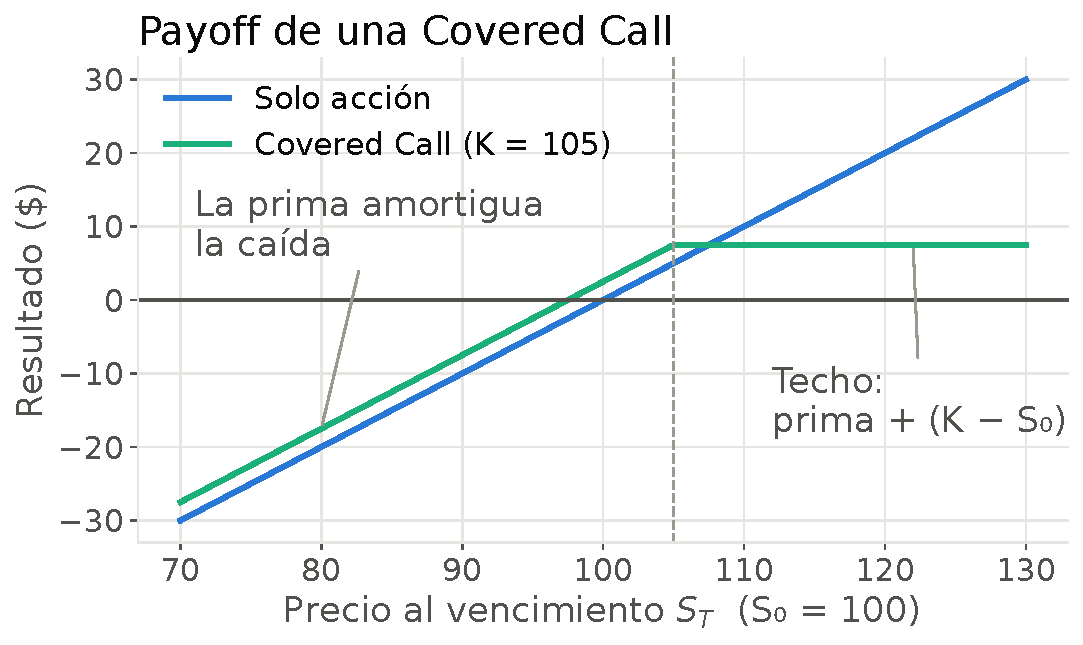
\includegraphics[width=\linewidth]{figures/01_payoff.pdf}
  \end{minipage}\hfill
  \begin{minipage}[c]{0.33\linewidth}
    La pregunta de fondo es simple:
    \begin{itemize}[leftmargin=*, itemsep=2mm, topsep=2mm]
      \item \textbf{\iq{}Esa renta compensa lo que se resigna?}
      \item Y si no siempre lo hace, \textbf{\iq{}un buen pronóstico de volatilidad puede decirnos cuándo conviene vender la call y cuándo no?}
    \end{itemize}
  \end{minipage}
}

\begin{columns}
% =====================================================================  COLUMNA 1
\column{0.34}

\block{Pregunta e hipótesis}{
  La prima depende de la \textbf{volatilidad implícita} (IV). Si después el mercado se mueve menos, el vendedor gana.
  \vspace{3mm}
  \innerblock{Hipótesis}{\centering Vender la call \textbf{solo si} nuestro pronóstico $\hat\sigma$ es \textbf{menor} que la IV \textbf{de esa call}, IV$(K)$.}
  \vspace{4mm}
  Comparamos contra \textbf{Buy \& Hold}, \textbf{CC estático} y \textbf{CC siempre OTM} (sin modelo), controlando el sobreajuste con el \textit{Deflated Sharpe}.
}

\block{Método}{
  \begin{center}
  \begin{tikzpicture}[node distance=4mm, every node/.style={font=\large},
     box/.style={draw=colorOne, fill=white!94!colorOne, rounded corners=3mm, thick, align=center, text width=0.76\linewidth, minimum height=10mm},
     hl/.style={box, draw=cMod, fill=cMod!10},
     arr/.style={-{Latex[length=4mm]}, very thick, color=ink2}]
    \node[box] (a) {Retornos OHLC hasta \mbox{$t_0-1$}};
    \node[box, below=of a] (b) {5 modelos de volatilidad $\to$ \textbf{ensamble} $\hat\sigma$};
    \node[hl, below=of b] (c) {Strike \mbox{$K=S_0\,e^{\,0{,}5\,\hat\sigma\sqrt{h/252}}$}};
    \node[hl, below=of c] (d) {IV de esa call: \mbox{$\text{IV}(K)=\text{IV}_{\text{índice}}\cdot(\SkewA-\SkewB\,x)$}};
    \node[hl, below=of d] (e) {\mbox{\iq{}$\hat\sigma<\text{IV}(K)$?\ $\Rightarrow$\ vender la call}\\ {\normalsize (si no, ese mes se tiene solo el activo)}};
    \node[box, below=of e] (f) {Black-Scholes $+$ ejercicio anticipado\\ antes del dividendo};
    \node[box, below=of f] (g) {P\&L del ciclo y drawdown diario};
    \foreach \i/\j in {a/b,b/c,c/d,d/e,e/f,f/g} \draw[arr] (\i) -- (\j);
  \end{tikzpicture}
  \end{center}
  {\small SPY y QQQ, \NCycles{} ciclos mensuales (ene-2008 a sep-2026). Decisión con datos hasta $t_0-1$; venta al cierre de $t_0$ (tercer viernes). $h$: ruedas del ciclo; $x=\ln(K/S)/(\text{IV}_{\text{índice}}\sqrt{T})$, $T$ en días corridos/365. IV del índice: VIX (SPY) o VXN (QQQ). Todo \textbf{walk-forward}; costo: 2\% de la prima.\\[1.5mm]\textbf{Validación:} el CC estático con opciones europeas (como el BXM) replica al ETF PBP: correlación \PBPcorr{}, rendimiento \PBPsim{} vs.\ \PBPbruto{} antes de comisiones.}

  \vspace{4mm}
  {\small\textbf{Los 5 modelos de volatilidad}\\[1mm]
  \renewcommand{\arraystretch}{1.25}
  \begin{tabular}{@{}p{0.24\linewidth}p{0.71\linewidth}@{}}
    \toprule
    \textbf{Modelo} & \textbf{Idea} \\ \midrule
    Rolling 21d & desvío de los últimos 21 retornos \\
    EWMA & $\sigma^2_t=\lambda\sigma^2_{t-1}+(1-\lambda)r^2_{t-1}$, $\lambda=0{,}97$ \\
    GJR-GARCH & $\sigma^2_t=\omega+(\alpha+\gamma\mathbf 1_{r<0})r^2_{t-1}+\beta\sigma^2_{t-1}$ \\
    HAR-RV & regresión sobre volatilidad diaria, semanal y mensual \\
    Kalman & log-varianza latente AR(1), estimada por MV \\
    Ensamble & promedio de las varianzas de los 5 modelos \\ \bottomrule
  \end{tabular}}


}

\block{Americanas vs.\ europeas}{
  \small
  \renewcommand{\arraystretch}{1.2}
  \begin{tabular}{@{}>{\raggedright\arraybackslash}p{0.2\linewidth}>{\raggedright\arraybackslash}p{0.39\linewidth}>{\raggedright\arraybackslash}p{0.35\linewidth}@{}}
    \toprule
    & \textbf{Americana}\newline SPY, QQQ (backtest) & \textbf{Europea}\newline SPX (skew y PBP) \\ \midrule
    Ejercicio & cualquier día & solo al vencimiento \\
    Dividendo & la call en el dinero se ejerce antes del ex-dividendo y el vendedor lo pierde & no aplica \\
    Paridad put-call & solo cotas & exacta \\ \bottomrule
  \end{tabular}

  \vspace{2mm}
  \normalsize
  SPY paga dividendo en la semana del vencimiento trimestral: el CC estático ATM sufrió \textbf{\SPYStatEarly{} ejercicios anticipados} y su rendimiento cae de \PBPsim{} (europea) a \textbf{\PBPsimAm{}} (americana), \textbf{$-$\EarlyCost{} por año}. El CC modelo, que casi no vende, solo \SPYModEarly{} veces.
}

% =====================================================================  COLUMNA 2
\column{0.33}

\block{\iq{}A qué IV se vende la call?}{
  \fig{03_iv_call_vs_realizada.pdf}
  \figcap{El VIX (naranja) suele estar por encima de la volatilidad realizada (azul). Pero la call que se vende (verde) cotiza por debajo de ambos.}
  \vspace{2mm}
  En SPY el VIX promedia \SPYIV{} y la volatilidad realizada \SPYRV: parece haber margen. Pero la \textbf{call vendida cotiza a \SPYIVcall} (QQQ: \QQQIVcall{} vs.\ \QQQRV{} realizada). El VIX está ``inflado'' por los \textbf{puts}, que son caros porque protegen de las caídas (\textit{skew}).
  \vspace{3mm}
  \key{\textbf{La prima de volatilidad está en los puts, no en las calls.}}
}

\block{Calidad de los pronósticos}{
  \fig{04_error_pronostico.pdf}
  \figcap{Error QLIKE fuera de muestra (menor es mejor). El Kalman (SPY: \SPYQlikeKalman) empata con la volatilidad implícita (\SPYQlikeIV); los modelos ingenuos son los peores. El ensamble (\SPYQlikeEns) queda cerca de los mejores.}

}

\block{Fase 1: features de volatilidad}{
  \fig[0.85]{fase1_ou_sscore.pdf}
  \begin{itemize}[leftmargin=*, itemsep=1.5mm]
    \item \textbf{Ornstein-Uhlenbeck} sobre $\ln\text{VIX}-\ln\text{VIX3M}$: half-life $\approx$\,\OUhalflife{} ruedas; estrés extremo ($s\ge2$) el \OUstress{} de los días.
    \item \textbf{Prima de varianza ex-ante}: VIX $-$ Yang-Zhang $=$ \VrpYZ{} (con Garman-Klass, \VrpGK: ignora el salto overnight).
    \item \textbf{Diferenciación fraccionaria} (log-precio, $d^*$ con 2007--2014): \DoptSPY{} en SPY y QQQ, \DoptNVDA{} en NVDA.
  \end{itemize}
}

% =====================================================================  COLUMNA 3
\column{0.33}

\block{Resultado: crecimiento de \$1}{
  \fig{06_crecimiento.pdf}
  \figcap{Escala logarítmica, retorno total (con dividendos). El CC modelo se superpone con el Buy \& Hold; vender siempre queda claramente abajo.}
}

\block{Estrategias comparadas}{
  \small
  \renewcommand{\arraystretch}{1.25}
  \setlength{\tabcolsep}{3.5pt}
  \begin{center}
  \begin{tabular}{@{}llrrrrrr@{}}
\toprule
& & \textbf{Total} & \textbf{CAGR} & \textbf{Vol.} & \textbf{Sharpe} & \textbf{MaxDD} & \textbf{Vende} \\ \midrule
SPY & Buy \& Hold & 712\% & 11.9\% & 18.5\% & 0.63 & -45\% & -- \\
SPY & CC estático ATM & 302\% & 7.7\% & 12.4\% & 0.56 & -33\% & 100\% \\
SPY & CC modelo & 565\% & 10.7\% & 16.5\% & 0.62 & -42\% & 84\% \\
\midrule
QQQ & Buy \& Hold & 1749\% & 16.9\% & 21.2\% & 0.78 & -47\% & -- \\
QQQ & CC estático ATM & 268\% & 7.2\% & 12.8\% & 0.51 & -37\% & 100\% \\
QQQ & CC modelo & 753\% & 12.2\% & 18.5\% & 0.65 & -47\% & 74\% \\
\bottomrule
\end{tabular}

  \end{center}
  {\footnotesize\color{ink2} CC siempre OTM: vende todos los meses con el mismo tipo de strike, usando la IV en lugar del modelo. MaxDD diario, con la call valuada a mercado. Sharpe y Sortino sobre excesos.}
}

\block{\iq{}Qué aporta el modelo?}{
  \small
  \begin{center}
  \renewcommand{\arraystretch}{1.25}
  \begin{tabular}{@{}lcc@{}}
    \toprule
    \textbf{CC modelo menos\ldots} (pp/año) & \textbf{SPY} & \textbf{QQQ} \\ \midrule
    Buy \& Hold & \SPYVsBH{} {\footnotesize\SPYVsBHCI} & \QQQVsBH{} {\footnotesize\QQQVsBHCI} \\
    CC siempre OTM & \SPYVsOTM{} {\footnotesize\SPYVsOTMCI} & \QQQVsOTM{} {\footnotesize\QQQVsOTMCI} \\
    CC estático ATM & \SPYVsStat{} {\footnotesize\SPYVsStatCI} & \QQQVsStat{} {\footnotesize\QQQVsStatCI} \\ \bottomrule
  \end{tabular}
  \end{center}
  {\footnotesize\color{ink2} Bootstrap estacionario, IC 95\%.}\\[2mm]
  El modelo vende solo el \textbf{\SPYModSold} de los meses en SPY (\QQQModSold{} en QQQ). Le gana a vender siempre, pero \textbf{no se distingue del Buy \& Hold} (probabilidad de superarlo: \SPYPSRactivo{} y \QQQPSRactivo{}, tras \NTrials{} configuraciones probadas).
}

\block{Conclusiones}{
  \begin{itemize}[leftmargin=*, itemsep=2mm]
    \item \textbf{Vender calls todos los meses rindió menos que quedarse con el índice:} la call ATM restó \SPYStatAporte{} por año en SPY y \QQQStatAporte{} en QQQ.
    \item \textbf{\iq{}Por qué?} La ``prima de volatilidad'' del VIX es el precio del seguro contra caídas (los puts). Las calls se venden baratas: a \SPYIVcall{}, cuando el mercado después se movió \SPYRV.
    \item \textbf{Un buen pronóstico sirve, pero para saber cuándo no vender.} Bien planteado, el modelo casi nunca vende y termina igual que el Buy \& Hold.
    \item \textbf{En la práctica:} en índices, la Covered Call no se justifica por la prima; si se usa, que sea sabiendo que cuesta rendimiento.
  \end{itemize}
  \vspace{2mm}
  {\small \textbf{Limitaciones}: skew calibrado con un solo período (jun--sep 2026) y aplicado también a QQQ; precios teóricos con costo fijo; solo 2 activos; las features de la fase 1 no entran en la decisión de venta. El ejercicio anticipado le cuesta \EarlyCost{} por año al CC estático sobre SPY.}
}
\end{columns}
\end{document}
